\documentclass{article}
\usepackage[top=2cm,bottom=2cm,left=2cm,right=2cm]{geometry}
\usepackage{amsmath, amssymb, amsthm}
\usepackage{ebproof}
\usepackage{hyperref}
\usepackage{csquotes}
\usepackage{tikz}
\usetikzlibrary{positioning}
\usetikzlibrary{shapes}

\usepackage{datetime}
\newdateformat{petsa}{\the\day\ \shortmonthname[\the\month] \the\year}

\newtheorem{definition}{Kahulugan}[section]
\newtheorem{theorem}{Teyorem}[section]
\newtheorem{lemma}[theorem]{Lema}
\newtheorem{problem}[theorem]{Problema}
\renewcommand{\abstractname}{Abstrak}
\renewcommand{\refname}{Sanggunian}

\title{Ilang mga Talâ sa Balintuna at Parakonsistensiya}
\author{poypoyan}
\date{25 Dec 2025}   % \petsa\today

\begin{document}

\maketitle

\begin{abstract}
Ito'y isang pagtitipon at saka paglalahad ng ilang mga talâ sa aking talaarawan patungkol sa balintuna (paradox) at pangangatuwiran kahit may (mga) kontradiksiyon.
\end{abstract}

\section{Isa pang Anyo ng Balintuna (09/09/2024)}
Noong isinulat ko ang papel patungkol sa diyagonalisasyon\cite{diagonal}, napaisip ako kung ang ibang kabalintunaan ay umaayon doon. Sa pagkakaalala ko, ang Balintuna ng Sinungaling ay oo, at gayundin ang kay Russell. Subali't para bagáng hindi sa Balintuna ng Káya ang Lahat (Omnipotence Paradox). At ngayon, may ideya na ako sa istruktura niyon at ng isa pa. Ganito ang nangyayari: may 2 o higit pang uri (class) na may dulot sa isa't isa.

\begin{center}
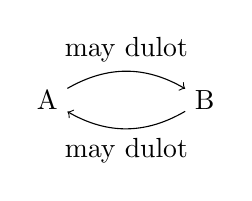
\begin{tikzpicture}[node distance = 1cm]
    \node (1) at (-1, 0) {A};
    \node (2) at (1, 0) {B};
    \draw[->] (1) to [bend left] node [midway,above]{may dulot} (2);
    \draw[->] (2) to [bend left] node [midway,below]{may dulot} (1);
\end{tikzpicture}
,
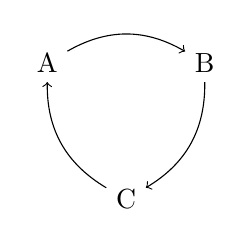
\begin{tikzpicture}[node distance = 1cm]
    \node (1) at (-1, 0) {A};
    \node (2) at (1, 0) {B};
    \node (3) at (0, -1.732) {C};
    \draw[->] (1) to [bend left] (2);
    \draw[->] (2) to [bend left] (3);
    \draw[->] (3) to [bend left] (1);
\end{tikzpicture}
,\ \ldots
\end{center}

At may ``idinidiin" na lagay sa lahat ng nasa $B$ ang isa sa $A$, datapwa't may isa sa $B$ na nagdudulot ng lagay na sumasalungat sa naunang lagay! Mabalik na táyo sa balintuna ng káya ang lahat, at suriin iyon. Ang dalawang uri doon ay \underline{Pahayag} at \underline{Gawain}:

\begin{center}
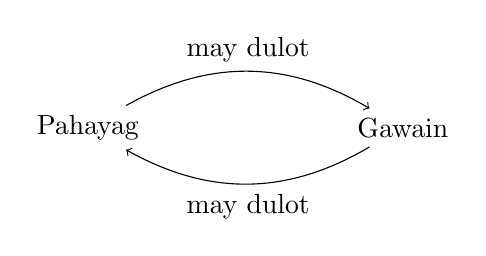
\begin{tikzpicture}[node distance = 1cm]
    \node (1) at (-2, 0) {Pahayag};
    \node (2) at (2, 0) {Gawain};
    \draw[->] (1) to [bend left] node [midway,above]{may dulot} (2);
    \draw[->] (2) to [bend left] node [midway,below]{may dulot} (1);
\end{tikzpicture}
\end{center}

\noindent\underline{Unang lagay:} Mula sa pahayag, ang ``pag-iral ng isang maykáyang gawin ang lahat" ay bubuhat ng potensiyal na pagkatapós ng anumang gawain.\\
\underline{Sumasalungat na lagay:} ang pahayag sa bato bílang ``di mabuhat-buhat ninuman". Ito ay sumasalungat sa \textit{isang} pahayag lang (``\ldots káyang gawin ang lahat"). Ano ang sanhi nito? Ang pagtapos sa paglikha ng bato, na isang gawain!

Sa kasong ito, ang pagdiin ng lagay \textit{sa lahat} ay di nasa lahat ng uri; \underline{di-pantay} ang itatawag ko rito. Ang sumusunod na balintuna ay isang halimbawa naman ng \underline{pantay}: Ang Balintuna ng Mangyayari kung Nagtagpo ang Di Mapigil-pigil sa Lakas at Di Magalaw-galaw na Bagay (Unstoppable Force Meets an Immovable Object). Nasa ngalan na ang dalawang uri (Lakas at Bagay) at ang dalawang lagay na idinidiin: ``di mapigil-pigil" = walang bagay na makapipigil, at ``di magalaw-galaw" = walang lakas na makagagalaw.

\section{Natatángang mga Balintuna (06/12/2024)}
Minsan talaga sa buhay ay may pinananatiling balintuna sa isipan na para bang tinatangan ito. Di na ito maipagkakaila. Ngayon, bakit? Ano-anong mga kinikilos natin sa isipan at natatangan ang balintuna? Di na rin maipagkakaila na hangga't maaari ay ayaw natin ng balintuna, batid man itong pagkaayaw o hindi. Ngayon, maglalahad ako ng dalawang halimbawa ng pagtangan ng balintuna:
\begin{enumerate}
\item Sa pisikang teyoretikal, isang litaw na suliraning di pa nalulutas ang ``pagsasama" ng dalawang teyorya, ang Kuwantum na Mekaniks at Pangkalahatang Relatibidad. Basta ang nauna ay mainam na pampaliwanag sa mga pinakamaliliit na tipik, subali't ang nahulí ay sa mga pinakamalalaki tulad ng bituin, galaksiya, mga pang-agham-tálà kumbaga. Ngayon, alam na kasi ng mga nagpipisika na may balintuna sa pagitan ng dalawa; di maaaring sabay na tama ang dalawa! Gayunman, ginagamit pa rin ang dalawa at di tinapon sa limot. Kunsabagay, may napakadaming kumpirmasyon pasasa dalawa, at napakaraming teknolohiyang inimbentong may gabay ng dalawa.
\item Ito'y lalong praktikal, malápit sa trabahong salukoy, at sa katunaya'y isinulat ko na (29/04/2024) at patungkol din sa parakonsistensiya:
\begin{quote}
\ldots Para bagá yaong tahimik lang kung gumagana ang sistema, datapwa't dádaíng na, nanghihingi ng masisisihan, kung hindi na gumagana!
\end{quote}
Ang halimbawang naiisip ko ay programa (sa kompiyuter). Kahit di tuluyang sinubok, o batid na malamáng ay may sira, maaaring gamitin pa rin iyon.
\end{enumerate}
Mula sa dalawang halimbawa, napagtanto kong di dahil lang sa may balintuna nang nahulo mula sa kaisipan, di na kapaki-pakinabang iyon. Di talaga natin tuwirang tinatangan ang mga balintuna, bagkus tinatangan ang napakikinabangang kaisipan. Naisip ko rin ngayon na ang matitirang konsistent sa lohikang parakonsistent ay ang pangangatuwiran natin sa mga teyorya, ugnayan sa pagitan ng mga iyon, at mga pamamaraan ng pagtatanggal ng kontradiksiyon sa mga iyon kung mayroon man.

\section{Isang Lohikang Parakonsistent (27/09/2025)} \label{paracon}
Tingin ko nahanap ko na ang pakaiibigin kong lohikang parakonsistent, at marahil ito ang pinakasimpleng pagbabago mula sa lohikang klasikal: magsimula sa karaniwang semantiks ng lohikang klasikal, ang talahanayan ng mga katotohanan (truth table), at ang tanging pagbabago lang ay paghuhulog ng $\Gamma\models\varphi$:

\begin{quote}
$\Gamma\models\varphi$ kung ang \underline{lahat ng proposisyonal na baryabulo ng $\varphi$ ay mula sa $\Gamma$}, at sa lahat ng $\mathcal{M}$ nks\footnote{na kung saan (such that)} $\mathcal{M}\models\Gamma$, aydi $\mathcal{M}\models\varphi$.
\end{quote}

Ang nakasalungguhit ang bago. Iyon na iyon! Paano nito natanggal ang ex falso ($\Gamma, \varphi, \neg\varphi\models\gamma$)? Sa kaso ng proposisyonal na lohika (wala munang $\forall$ at $\exists$), dapat ang lahat ng baryabulo sa konklusiyon ay mga baryabulo rin ng premis! Sa halip ng pagsabog ay $\neg A$ at $A$ na lámang ang mga konklusiyon sa mga premis na $A, \neg A$. May kondisyon na rin sa pagpapasok ng $\vee$ ($\Gamma, \varphi\models\varphi\vee\gamma$) na dapat nasa premis ang mga baryabulo ng $\gamma$. At ang hulí kong sasabihin, paano na ang simbolo ng katotohanan $\top$? Tanggal rin ba ang $\top\models\varphi\wedge\neg\varphi\rightarrow\gamma$? Hindi, ngunit kailangang maging ``daglat" ang $\top$ ng pormulang gawa sa mga baryabulo: $$\top(A) = A \vee \neg A$$ $$\top(A,B) = (\neg A \wedge \neg B) \vee (\neg A \wedge B) \vee (A \wedge \neg B) \vee ( A \wedge B)$$at alam na ang pagtutuloy. Ibig ko na ito kasi bukod sa malápit sa lohikang klasikal, nakikita ko nang hindi mahirap mangatuwiran gamit ito---alalahanin lámang ang mga baryabulo sa magkabilang banda ng $\models$!

Ang susunod na gagawin ay bumuo ng listahan ng mga tuntunin ($\Gamma\vdash\varphi$) at patunayan ang mga teyorem ng katinuan (soundness) at kabuuan (completeness).

Karagdagang talang wala sa talaarawan: Lumitaw na lalo ang pagkakaiba ng $\vdash$ at ng $\rightarrow$, na madalas napag-iisa. Kung ang $\rightarrow$ ay materyal na implikasiyon pa rin ($A\rightarrow B$ = sa lahat ng mga ``kalagayan" nks totoo ang $A$, totoo rin doon ang $B$), sinasagisag naman ng $\vdash$ ang mga \textit{maaaring kilos natin sa pangangatuwiran}. Sinasabi ng bagong $\models$ na kapagka nakatagpo ng kontradiksiyon, humingang malalim at hindi táyo tutuloy sa pangkokonklusiyon ng kung ano-ano, at ito naman talaga ang ating kinikilos, hindi ba?

\section{Pagkabukod ng Kaganapan, Kayamanan ng Mangasasabi (19/10/2025)}
Ayto ang isa pang ibig sabihin ng semantiks ng bagong tala kong lohikang parakonsistent (27/09/2025): pagkabukod (isolation) ng ``kaganapan" sa mga tipón ng pahayag (na tinatawag na ``teyorya" sa larang ng lohikang matematikal). Ito'y sapagka't walang napakalayo sa teyoryang proposisyon ang lilitaw na bigla sa konklusyon, bagkus ang mga konklusyon'y bágong pagsasama-sama lamang ng mga nasa loob ng teyorya. Sa palarawan:

\begin{center}
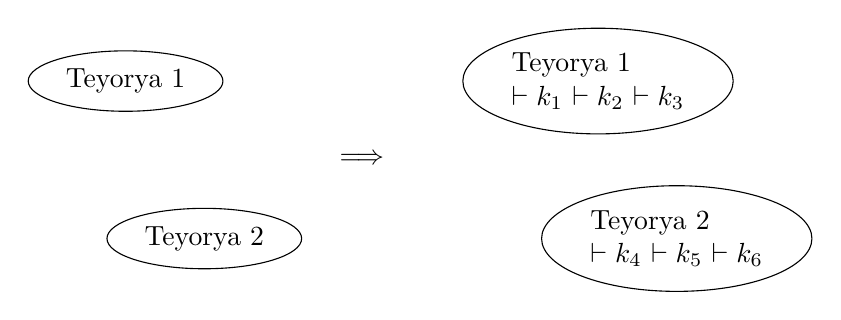
\begin{tikzpicture}[node distance = 0.5cm]
    \node (1) at (-3,1)   [draw, ellipse]   {Teyorya 1};
    \node (2) at (-2,-1)   [draw, ellipse]   {Teyorya 2};
    \node (i) at (0, 0) {$\implies$};
    \node (1n) at (3,1)   [draw, ellipse, align=left]   {Teyorya 1\\$\vdash k_1$ $\vdash k_2$ $\vdash k_3$};
    \node (2n) at (4,-1)   [draw, ellipse, align=left]   {Teyorya 2\\$\vdash k_4$ $\vdash k_5$ $\vdash k_6$};
\end{tikzpicture}
\end{center}

Kahit $k_5 = \neg k_6$, di sasabog ang kontradiksyon palabas ng Teyorya 2. Kahit $k_1 = \neg k_5$, di sasabog ang kontradiksyon palabas ng ``teyoryang" binubuo ng kasalukuyang tinatalakay (ang pagsasama ng dalawang teyorya).

Malamáng naisulat ko na rin noon pa ang pahayag na nabása ko mandin sa isang aklat na maganda kung may masasabi táyo sa (iba't ibang) kontradiksiyon---payak at masalimuot, tulad ng ibang paksa---di tulad na giit ng lohikang klasikal na (halos) wala kasi lahat ay mahuhulo mula sa kontradiksyon. O ngayong may lohika nang maganda, nasaan ang mangasasabi? Wala pa akong halimbawa paririto, datapwa't may pahiwatig sa larawan sa itaas: mahalaga ang bakod ng mga teyorya sa pag-iiba; ang ``tinagusang bakod" ng kontradiksyon ang pinagkaiba ng $k_1 = \neg k_5$ sa $k_5 = \neg k_6$.

\begin{center}
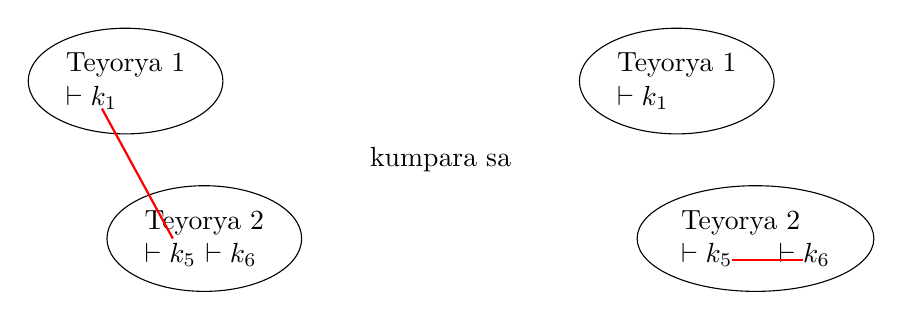
\begin{tikzpicture}[node distance = 0.5cm]
    \node (1n) at (-4,1)   [draw, ellipse, align=left]   {Teyorya 1\\$\vdash k_1$};
    \node (2n) at (-3,-1)   [draw, ellipse, align=left]   {Teyorya 2\\$\vdash k_5$ $\vdash k_6$};
    \draw[thick, draw=red] (-4.3, 0.65) -- (-3.4, -1);
    \node (i) at (0, 0) {kumpara sa};
    \node (1n) at (3,1)   [draw, ellipse, align=left]   {Teyorya 1\\$\vdash k_1$};
    \node (2n) at (4,-1)   [draw, ellipse, align=left]   {Teyorya 2\\$\vdash k_5$~~~~~$\vdash k_6$};
    \draw[thick, draw=red] (3.7, -1.27) -- (4.6, -1.27);
\end{tikzpicture}
\end{center}

Idagdag sa lohikang maganda ang iba't ibang pagbubuo't ugnayan ng mga teyorya (na mga tipón mandin; alalahanin ang $\cup$, $\cap$, \ldots) at ang pagiging anuman ng dami ng pahayag na bumubuo ng kontradiksyon (tingnan din ang mga ``uri" sa unang seksiyon sa itaas) at natatanaw ko na ang kayamanan ng mangasasabi!

\section{Ang Sikwent na Kalkyulus para sa \ref{paracon} (07/06/2026)}
Ang sistema ay gayundin sa sistemang \textbf{LK} ni Gentzen para sa lohikang klasikal, subalit may pagbabago lang sa mga sumusunod na tuntunin:
\begin{itemize}
    \item Paghihina sa kanan ($WR$):
        \begin{prooftree}
        \hypo{\Gamma \vdash \Delta}
        \infer1{\Gamma \vdash \varphi, \Delta}
        \end{prooftree}
    \item $\vee$ sa kanan ($\vee R$):
        \begin{prooftree}
        \hypo{\Gamma \vdash \gamma, \Delta}
        \infer1{\Gamma \vdash \varphi \vee \gamma, \Delta}
        \end{prooftree}
    at
        \begin{prooftree}
        \hypo{\Gamma \vdash \gamma, \Delta}
        \infer1{\Gamma \vdash \gamma \vee \varphi, \Delta}
        \end{prooftree}
    \item $\rightarrow$ sa kanan ($\rightarrow R$):
        \begin{prooftree}
        \hypo{\Gamma, \varphi \vdash \gamma, \Delta}
        \infer1{\Gamma \vdash \varphi \rightarrow \gamma, \Delta}
        \end{prooftree}
    \item $\neg$ sa kanan ($\neg R$):
        \begin{prooftree}
        \hypo{\Gamma, \varphi \vdash \Delta}
        \infer1{\Gamma \vdash \neg \varphi, \Delta}
        \end{prooftree}
\end{itemize}

Markahan ang proposisyong may $\varphi$ sa ibaba (hal.,
        \begin{prooftree}
        \hypo{\Gamma, \varphi \vdash \Delta}
        \infer1{\Gamma \vdash (\neg \varphi)^{*}, \Delta}
        \end{prooftree}
) kung may proposisyonal na baryabulo doon na wala sa $\Gamma$. Sa anumang susunod na tuntuning gagamitin, markahan pa rin ang resultang proposisyong may $\varphi$, \textit{maliban lang kung nilipat ang buong iyon sa kaliwa (sa pamamagitan ng $\rightarrow L$  o $\neg L$)}. Hindi wasto ang patunay kung may marka ang hulíng sikwent. Halimbawa, ang sumusunod ay wasto:
\[
\begin{prooftree}
    \hypo{}
    \infer1[$(Id)$]{A \vdash A}
    \infer1[($\vee R$)]{A \vdash (A \vee B)^{*}}
    \infer1[($\rightarrow R$)]{\vdash (A \rightarrow (A \vee B))^{*}}
    \infer1[($\neg L$)]{\neg(A \rightarrow (A \vee B)) \vdash}
\end{prooftree}
\]

\begin{theorem}
Ang pagbabagong ito ay maayos (sound) at buo (complete) ayon sa pagbabago ng semantiks sa \ref{paracon}.
\end{theorem}
\begin{proof}[Patunay]
Maayos na agad kasi ginagawang mali ng marka ang mga patunay nks sa hulíng sikwent nito, may baryabulo sa kanan ng $\vdash$ na wala sa kaliwa. Sa kabiláng bandá, dahil sa wala namang tinanggal na tuntunin sa bagong sistema ng patunay, ang patunay sa \textbf{LK} ng isang $\Gamma\models\varphi$ na umaayon sa bagong semantiks sa \ref{paracon} ay patunay na rin sa bagong sistema---minarkahan lang. Dahil sa kabuuan ng \textbf{LK} sa lohikang klasikal, magiging buo na rin ang bagong sistema.
\end{proof}

\bibliographystyle{plain}
\bibliography{balintuna}
\end{document}
